\begin{BPMN}{PROC-03}{Creación de una Unidad de Aprendizaje}{}
    \PCitem{Participantes}{}
    \PCitem{Objetivo}{}
    \PCitem{Interrelación con otros procesos}{}
    \PCitem{Proveedores}{}
    \PCitem{Entradas}{}
    \PCitem{Consumidores}{}
    \PCitem{Salidas}{}
    \PCitem{Precondiciones}{}
    \PCitem{Postcondiciones}{}
    \PCitem{Frecuencia}{}
    \PCitem{Tipo}{}
    \PCitem{Áreas de oportunidad}{}
\end{BPMN}
En la figura \hyperref[]{}
\begin{figure}[htbp]
	\begin{center}
		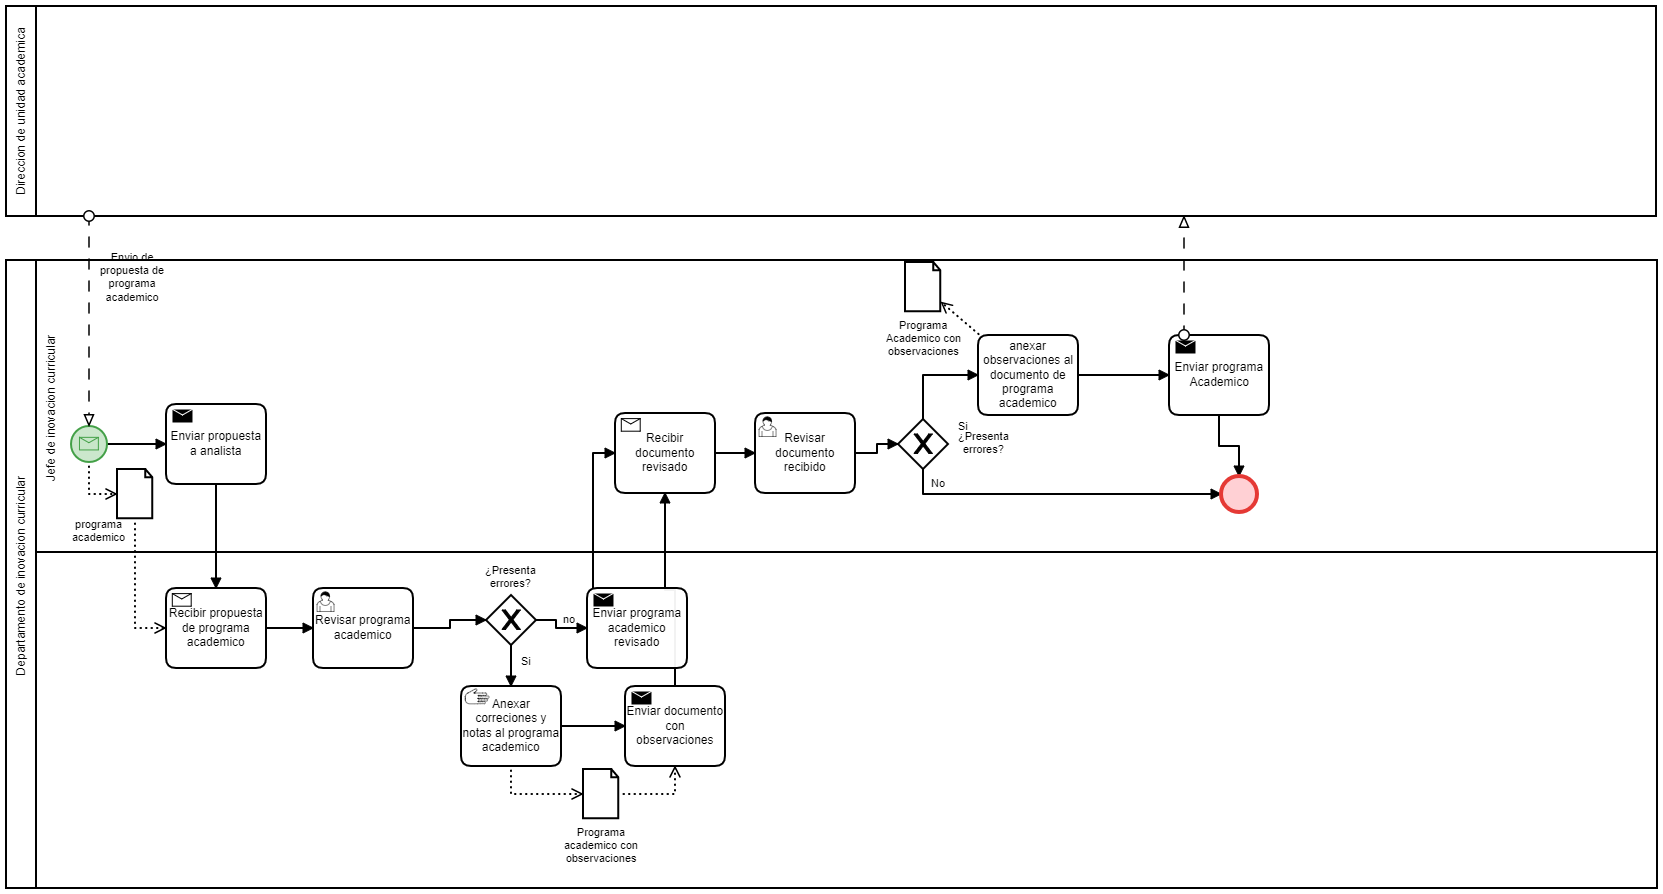
\includegraphics[width=.95\textwidth]{C1-DP/SP5/validarPA.png}
		\caption{}
		\label{fig:}
	\end{center}
\end{figure}